\documentclass{article}
\usepackage[utf8]{inputenc}
\usepackage{amsmath,amssymb,amsfonts}
\usepackage{amsthm}
\let\oldAA\AA
\renewcommand{\AA}{\text{\normalfont\oldAA}}
\usepackage[makeroom]{cancel}
\usepackage{graphicx}
\usepackage{caption}{\tiny }
\usepackage[affil-it]{authblk}
\usepackage{multirow}
\usepackage[table,xcdraw]{xcolor}
\usepackage{titlesec}
\usepackage{longtable}
\usepackage{wrapfig}
\usepackage{mathtools}
\usepackage{braket}
\usepackage{bm}
\usepackage{esvect}
\usepackage[colorlinks = true,
            linkcolor =  black,
            urlcolor  = blue,
            citecolor = blue,
            anchorcolor = blue]{hyperref}

\newcommand{\MYhref}[3][blue]{\href{#2}{\color{#1}{#3}}}%
\usepackage[
bookmarksopen,
bookmarksdepth=2,
breaklinks=true
]{hyperref}
\usepackage{arxiv}
\usepackage[utf8]{inputenc} % allow utf-8 input
\usepackage[T1]{fontenc}    % use 8-bit T1 fonts
\usepackage{hyperref}       % hyperlinks
\usepackage{url}            % simple URL typesetting
\usepackage{booktabs}       % professional-quality tables
\usepackage{amsfonts}       % blackboard math symbols
\usepackage{nicefrac}       % compact symbols for 1/2, etc.
\usepackage{microtype}      % microtypography
\usepackage{lipsum}		% Can be removed after putting your text content
\usepackage{graphicx}
\usepackage{natbib}
\usepackage{doi}
\renewcommand\refname{}
\renewcommand*\contentsname{}



\title{Plazma Hızlandırıcıları}

\date{4 Aralık 2021}


\author{ \href{https://orcid.org/0000-0002-1684-9602}{
\includegraphics[scale=0.06]{orcid.pdf}\hspace{1mm}Halil Kolatan} \\
	Ankara Üniversitesi\\
	Fen Fakültesi 
	Fizik Bölümü }\\
	%halilkolatan@gmail.com	}
% Uncomment to remove the date

% Uncomment to override  the `A preprint' in the header
%\renewcommand{\headeright}{Technical Report}
%\renewcommand{\undertitle}{Technical Report}
%\renewcommand{\shorttitle}{\textit{arXiv} Template}

%%% Add PDF metadata to help others organize their library
%%% Once the PDF is generated, you can check the metadata with
%%% $ pdfinfo template.pdf
\hypersetup{
pdftitle={Plazma Hızlandırıcıları},
pdfsubject={Plasma physics},
pdfauthor={Halil }
pdfkeywords={Plazma},
}

\begin{document}
\maketitle
\begin{abstract}
\tableofcontents
\end{abstract}
\section{Giriş}
 Parçacık fiziğinde keşif arayışı her zaman mümkün olan en yüksek enerjilerde deneyler gerektirmiştir. Yüksek enerjili parçacık hızlandırıcılar ise şimdiye kadar parçacık fiziğinin doğasını anlamak için vazgeçilmez bir araç olmuştur. Parçacık demetlerini çok yüksek enerjiyle hızlandırmak, bu demetleri çarpıştırmak ve bu çarpışmaların oluşturduğu parçacıkları tespit etmek için yeni teknikler geliştirilmiştir. Standart Modelin (SM) ötesinde, yükseltilmiş bir enerji seviyesinde yeni parçacıklar arayışını sürdürebilecek bir tesis yaratmak için teknikte daha fazla ilerleme gereklidir. Günümüzde hızlandırıcılar, yaklaşık 100 MV/m ile sınırlı değerlere sahip elektrik alanlarını ayakta tutan metalik kaviteler kullanmaktadır. Aşırı hızlanan gradyanları destekleme yetenekleri nedeniyle, plazma ortamı yakın zamanda gelecekteki kavite benzeri hızlandırıcı yapılar için önerilmiştir. Bu araştırma ödevi, birçok uygulama için çok uygun hale getiren bir dizi parametre ile yüksek kaliteli parçacık demetlerinin üretilmesine izin veren lazer veya parçacık demetleri tarafından yönlendirilen plazma hızlandırıcılarını  incelemektedir.
 
  \newpage
  
   \section{Plazma Hızlandırıcıları}
   
   Geleneksel parçacık hızlandırıcıları büyük ve pahalı makinelerdir. Plazma tabanlı hızlandırıcılar olası kompakt bir alternatiftir. Plazma hızlandırıcılar, parçacıkların enerji kazanmak için "sörf" yaptığı plazma dalgaları üretir. Bir plazma akıntısının arkasına bir demet parçacık yerleştirildiğinde, dalga sörfçüleri gibi hızlanır.
 
  \begin{figure}[h!]
 \centering
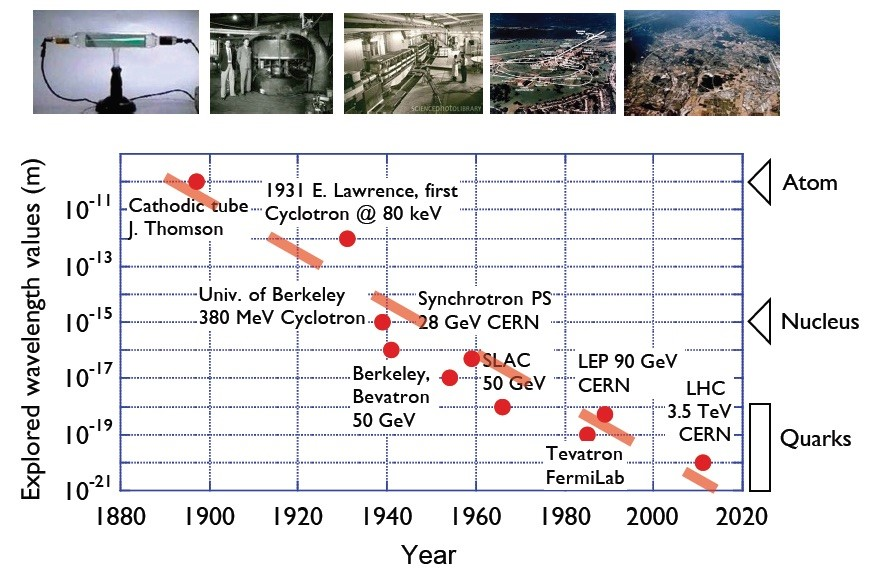
\includegraphics[width=9cm]{ss23.png}
\caption*{Şekil 1. Hızlandırıcıların gelişimi ve başlıca keşifleri [1].}
	\end{figure}

Lazerle çalışan plazma tabanlı hızlandırıcılar, ilk olarak kırk yıl önce Tajima ve Dawson tarafından önerildi. 2001 yılında vefat eden Dawson, plazma atım dalgası hızlandırıcısı, lazer akıntı alanı (wakefield)$^1$ hızlandırıcısı ve foton hızlandırıcısı dahil olmak üzere bu alandaki ilk gelişmelerin çoğundan sorumluydu. Çalışmalarının anahtarı, geleneksel hızlandırıcıların dayandığı süper iletken radyofrekans boşluklarının aksine, bir plazmanın iyon ve elektron yüklerini yüksek yoğunluklu bir lazerle ayırarak oluşturulabilen 100 GV m$^{-1}$ ve daha büyük muazzam elektrik alanlarını destekleyebilmesidir [2,3].
\footnotetext[1]{bk. \MYhref[magenta]{https://hpfbu.web.cern.ch/HPFBU/Sozluk.html}{\textit{Hızlandırıcı Fiziği Sözlüğü}}}


 \begin{figure}[h]
 \centering
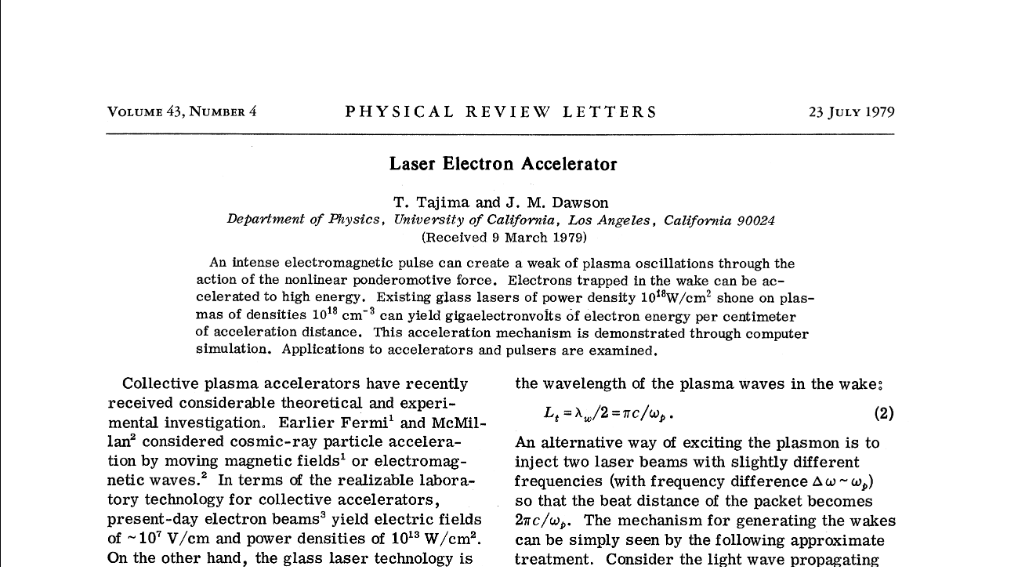
\includegraphics[width=10cm]{makale.png}
\caption*{Şekil 2. Tajima ve Dawson tarafından önerilen ilk plazma tabanlı hızlandırıcı çalışması [2].}
	\end{figure}
	
1985'te Chen ve Dawson, plazma akıntılarını sürmek için bir demet elektron ışını kullanmayı önerdiler. Kısa bir süre sonra, düşük enerjili elektron ışını sürücüleri kullanılarak Parçacık Akıntı Alanı Hızlandırma (PWFA) ile ilgili ilk deneyler gerçekleştirildi.  İlk deneylerde akıntı alanlarını sürmek için uzun bir lazer darbesi kullanıldı ve 1990'larda plazma akıntı alanı ivmesi ilkesini gösterdi.  Bu gelişmeler gerilmiş darbe amplifikasyonunun (chirped pulse amplification) icadı sayesinde gerçekleşmiştir. Strickland ve Mourou’nun icat ettiği gerilmiş darbe amplifikasyonu tekniği sayesinde, bilinen en şiddetli optik darbelerin üretimi mümkün olmuştur. 1985 yılında geliştirilen teknik, lazer darbelerinin optik kazanç ortamına zarar vermeden amplifikasyonunu sağlayan öncü bir tekniktir. Bu teknik 2019 yılında Nobel Fizik Ödülü'ne layık görüldmüştür [1,4].

\newpage

 \begin{figure}[h]
 \centering
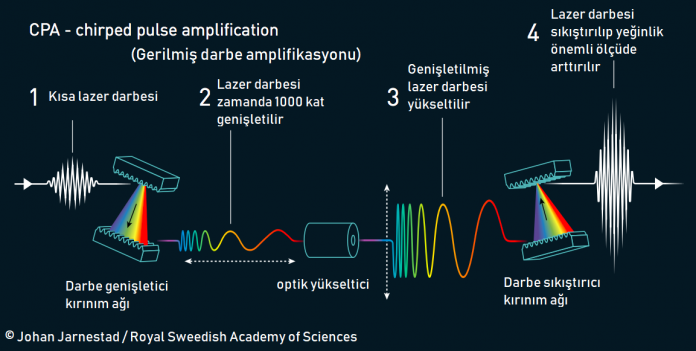
\includegraphics[width=10cm]{CPA-tr2-696x351.png}
\caption*{Şekil 3. Gerilmiş Darbe Amplifikasyonu (CPA) [5].}
	\end{figure}
	
\subsection{Plazma}

Plazma, kollektif davranış sergileyen, yüklü (+ ve -) ve nötral parçacıklardan oluşan hemen hemen nötral bir gazdır.

\begin{itemize}
    \item \textbf{Hemen hemen nötrallik:} Pozitif ve negatif yüklerin hemen hemen eşit olması demektir.
    \item \textbf{Kollektif davranış: } Sadece yerel şartlara bağlı olmayan, uzak bölgelerdeki şartlara da bağlı olan hareketi anlıyoruz. Kolleftif davranıştan dolayı; bir plazma dış etkilere uyma eğiliminde değildir, genelikle kendi aklı varmış gibi davranır.
\end{itemize}

 \begin{figure}[h]
 \centering
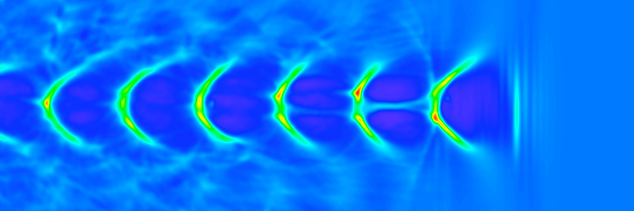
\includegraphics[width=8cm]{plasma_wave.png}
\caption*{Şekil 4. Bir plazma dalgası ($ \sim 50 \mu m;  \sim 100 \textrm{GV/m}$).}
	\end{figure}
 
 
 \subsection{Plazma Akıntı Alanı Hızlandırıcısı}
 
 Plazma parçacıklarının toplu hareketiyle oluşturulan alanlara plazma akıntı alanları denir.
 
 \begin{figure}[h]	
 \centering
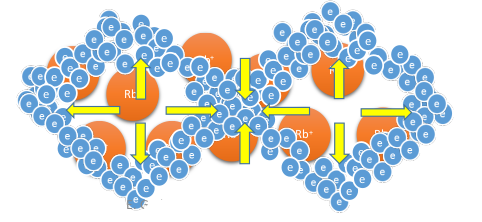
\includegraphics[width=11cm]{wakefield.png}
\caption*{Şekil 5. Plazma akıntı alanı [6].}
	\end{figure}

 Yüklü parçacıkları hızlandırmak için boyuna elektrik alanı gerekmektedir. Sürücü demetinin enine elektrik alanını plazmada boyuna bir elektrik alanına dönüştürmek için plazma kullanılmaktadır. Böylelikle ne kadar çok enerji varsa, bu plazma akıntı alanı o kadar uzun (mesafe açısından) sürülebilir.
 
 
\newpage

 \begin{figure}[h]
 \centering
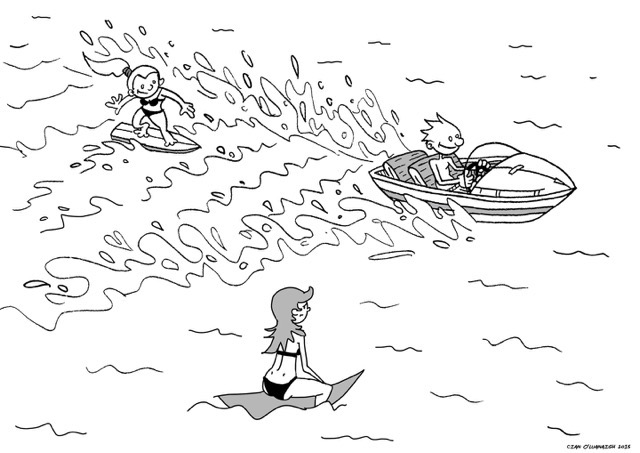
\includegraphics[width=11cm]{surfing.png}
\caption*{Şekil 6. Plazma akıntı alanı için bir analoji [6].}
	\end{figure}
	
Bu analojide su $\Rightarrow$ plazma, bot $\Rightarrow$ parçacık demeti, sörfçü $\Rightarrow$ hızlandırılmış parçacık demetidir.
	
Bir bot suda hareket ettiğinde arkasında bir dalga oluşturur - bir "akıntı". Bu dalganın faz hızı sadece botun hızı kadardır. Böylece arkasında güçlü bir dalga sürmek için plazmada c'ye yakın bir hızda hareket eden bir lazer atması kullanabiliriz. Bu durumda dalga bir elektron plazma salınımı olmaktadır. 
\begin{align}
    \omega_{p} = \bigg( \dfrac{n_{0} e^{2}}{m_{e} \epsilon_{0}}  \bigg)^{\dfrac{1}{2}}
\end{align}
Bunlar yüksek frekanslı salınımlar olduğu için iyonlar hareket etmez ve çok güçlü elektrik alanları oluşmaktadır.

\subsection{Sürücü Kuvvet}
Ponderomotive kuvvet tarafından sürülen lazer akıntı alanı hızlandırıcıları için,

\begin{align}
    \dfrac{d\vv{p}}{dt} = - \dfrac{e^{2}}{2m_{e} \omega_{0}^{2}} \nabla \braket{E^{2}} = -\dfrac{e^{2}}{2m_{e}} \nabla \braket{A^{2}} = -\dfrac{1}{2} m_{e}c^{2} \nabla \braket{a^{2}}
    \end{align}
    
\subsection{Temel Plazma Parametreleri}

Yoğunluğu $n_{pe}$ olan bir plazma, plazma frekansı ile karakterize edilir,

\begin{align}
    \omega_{pe} = \sqrt{ \dfrac{n_{pe}e ^{2}}{m_{e} \epsilon_{0} }} \Rightarrow \dfrac{c}{\omega_{pe}} \qquad k_{pe} = \dfrac{\omega_{pe}}{c}
\end{align}

Bu, plazma salınımının bir dalga boyuna çevrilir,

\begin{align}
\lambda_{pe} = 2 \pi \dfrac{c}{\omega_{pe}} \Rightarrow \lambda_{pe} \approx 1 \textrm{ mm} \sqrt{\dfrac{10^{15} \textrm{cm}^{-3} }{n_{pe}}}    
\end{align}
 
 
\newpage
\section{Avantajları}
Plazma hızlandırıcılarnın, başlıca avantajları şunlardır: 
\begin{itemize}
    \item Günümüzde kullanılan geleneksel hızlandırcılar genellikle çok büyük bir tesise ihtiyaç duyarlar ve oldukça maliyetli iken plazma hızlandırıcıları çok daha küçük boyutlu ve maliyeti çok daha düşüktür.
\end{itemize}
 \begin{figure}[h]
 \centering
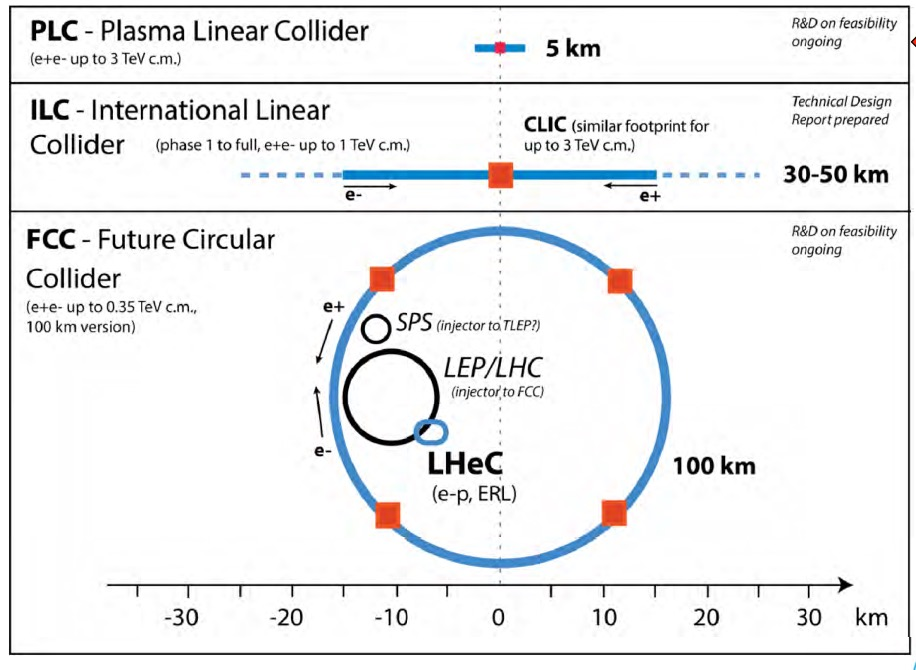
\includegraphics[width=7cm]{index.png}
\caption*{Şekil 7. Farklı tipteki çarpıştırıcılar ile plazma çarpıştırıcılarının karşılaştırılması [6].}
	\end{figure}
	\begin{figure}[h]
 \centering
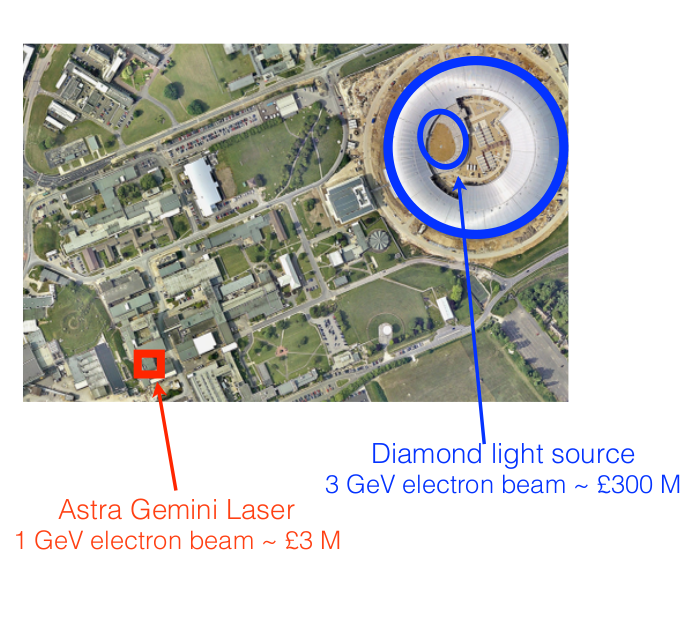
\includegraphics[width=8cm]{maliyet.png}
\caption*{Şekil 8. Maliyet karşılaştırılması.}
	\end{figure}
	\begin{itemize}
	    \item Küçük mesafelerde yüksek enerjilere çıkabilmektedir.
	\end{itemize}
\begin{itemize}
    \item Plazma hızlandırıcıları düşük maliyetli ve küçük boyutlu olduğu için araştırmalarda, üniversitelerde, ve hastanelerde rahatlıkla kullanılabilir.
\end{itemize}
\begin{itemize}
    \item Elektronlar $ \sim 100$ TW lazer ile $ \sim 1$ GeV'e kadar hızlandırılabilmektedir.
\end{itemize}
\section{Dezavantajları}
Plazma hızlandırıcılarının, başlıca dezavantajları şunlardır: 
\begin{itemize}
    \item Şuanki hızlandırıcı teknolojisinden çok daha az enerjilere ulaşabilmektedir. Gerçekçi çarpıştırıcı demet parametrelerine ulaşmak için çok ilerleme yapılması gerekmektedir.
\end{itemize}
\begin{itemize}
    \item Hızlanan alanlar <100 MV/m ile sınırlıdır. 
\end{itemize}
\begin{itemize}
    \item Metalik yapılarda, çok yüksek bir alan seviyesi yüzeylerin parçalanmasına yol açarak elektrik boşalması oluşturur.
\end{itemize}


\section{Plazma Hızlandırıcı Tesisleri}

Tablo 5.1 dünya çapındaki mevcut PWFA tesislerini özetlemektedir. AWAKE, CLEAR, Flash- Forward ve INFN SPARCLAB kullanımdayken, FACET-II, CLARA ve EuPRAXIA@SparcLAB şu anda yapım aşamasındadır. MAX IV, planlama ve tasarım aşamasındadır. Tesislere bağlı olarak, ana araştırma konuları farklılık gösterir ve PWFA, FEL ve diğer uygulamaları içerir. AWAKE dışında, tesislerde şu anda yüksek enerji fiziği uygulamaları ana odak noktası değildir. FACET-II ve SPARCLAB, pozitron demetleri sağlamak için tesislerini daha sonraki bir aşamada yükseltmeyi planlıyor [7].

 \begin{figure}[h]
 \centering
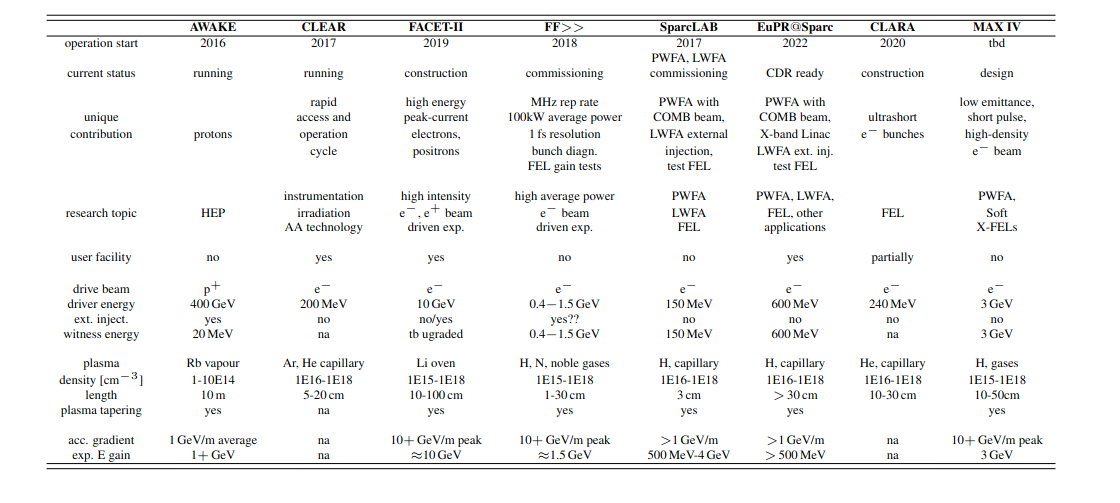
\includegraphics[width=16cm]{tablo1.png}
\caption*{Tablo 5.1 Dünya'daki mevcut plazma hızlandırıcıları tesisleri [7].}
	\end{figure}
	
	\begin{figure}[h]
 \centering
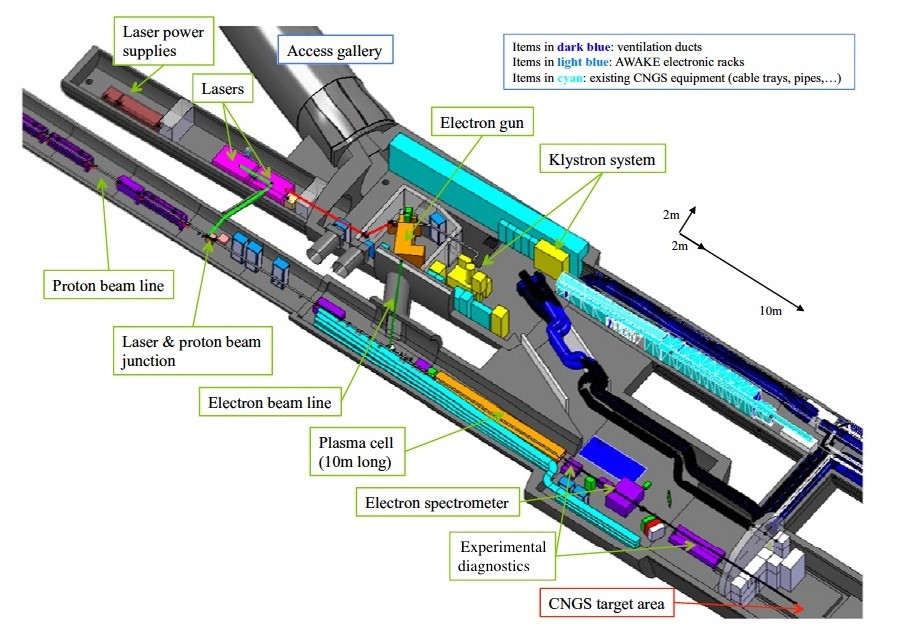
\includegraphics[width=10cm]{awake.png}
\caption*{Şekil 9. CERN-AWAKE deneyinin tasarımı [1].}
	\end{figure}
	
	
	
\clearpage

\section{Yeni Fizik Potansiyeli}	

Plazma bazlı, yüksek enerjili elektron-pozitron lineer çarpıştırıcı, geleneksel teknolojilere dayalı bir hızlandırıcıdan daha yüksek ışınlığa ve aynı zamanda daha kısa bir uzunluğa ve daha düşük maliyete sahip olan TeV enerji sınırına ($\geq 10$ TeV) ulaşabilir. Bu enerjilerde, yüzlerce GeV enerji aralığında önerilen çarpıştırıcıların kapsadığı alanın ötesinde fiziğe erişilebilir. Örneğin, Higgs bozonunun bazı özelliklerini araştırmak ve çoklu TeV kütleli yeni parçacıklar aramak veya olası ekstra uzay boyutlarının ipuçlarını ortaya çıkarmak mümkün olacaktır. Fizikçiler, 2030'ların ortalarına kadar plazma tabanlı, yüksek enerjili elektron-pozitron lineer çarpıştırıcı için bir tasarım geliştirmeyi amaçlıyorlar. Önümüzdeki 10 yıl boyunca, plazma tabanlı hızlandırıcıların temel zorluklarını ele almaya ve elektronları ve pozitronları yüksek demet kalitesiyle çoklu GeV aralığına hızlandırmaya çalışılacak.


\section{Kaynakça}

	\begin{thebibliography}{99}
	\bibitem{mano} Malka, V (2017). \textit{Plasma Wake Accelerators: Introduction and Historical Overview}. arXiv e-print. \MYhref[blue]{https://arxiv.org/abs/1705.09584}{\textrm{arXiv:1705.09584.}}  
	
	\bibitem{mano} Tajima, T.; Dawson, J. M. (1979). \textit{Laser Electron Accelerator}. Physical Review Letters, 43(4), 267–270. doi:10.1103/physrevlett.43.267.
	
	\bibitem{mano} Esarey, E.; Schroeder, C. B.; Leemans, W. P. (2009) \textit{Physics of laser-driven plasma-based electron accelerators}. Reviews of Modern Physics, 81(3), 1229–1285. doi:10.1103/revmodphys.81.1229.
	
	\bibitem{mano} Gschwendtner, E.; Muggli, P. (2019). \textit{Plasma wakefield accelerators.} Nat Rev Phys 1, 246–248. doi:0.1038/s42254-019-0049-z.
	
	\bibitem{mano}  (Dijital Görsel) \textit{2018 Nobel Fizik Ödülü: Lazer fiziğinde devrimsel iki buluş} Web sitesi: \url{https://sarkac.org/2018/10/lazer-fiziginde-devrimsel-iki-bulus/}. Erişim tarihi: 03.12.2021.
	
	\bibitem{mano} Gschwendtner, E. (2021). \textit{Plasma Wakefield Acceleration and the AWAKE Experiment} [PDF  belgesi]. Basic CERN Accelerator School. Web sitesi: \url{https://indico.cern.ch/event/1018359/contributions/4312244/attachments/2248469/3813952/2021-05-20-PlasmaWakefieldAcceleration-CAS.pdf} Erişim tarihi: 03.12.2021.
	
	\bibitem{mano} ALEGRO collaboration (2019). \textit{Towards an Advanced Linear International Collider}. arXiv e-print. \MYhref[blue]{https://arxiv.org/abs/1901.10370}{\textrm{arXiv:1901.10370.}}   



	\end{thebibliography}
	


\end{document}
